% !TEX root = ../Main.tex
\chapter{垂直关系}

垂直关系和平行关系一样，也分线线、线面、面面三层。三层之间靠判定定理（往下走）和性质定理（往上走）来回转换。下面把每一层常用的来源列清楚，标 $\blacktriangle$ 的是判定定理。

\section{直线之间（线线垂直）}

\state{线线垂直的来源}{
    \begin{enumerate}
        \item[(i)] 平面几何证法：矩形、等腰三角形的"三线合一"；
        \item[(ii)] 利用平行的传递性；
        \item[(iii)] $\blacktriangle$\ $\bc l_1\perp\alpha\\ l_2\subset\alpha\ec\ \Rightarrow\ l_1\perp l_2$；
        \item[(iv)] $\bc l_1\perp\alpha\\ l_2\parallel\alpha\ec\ \Rightarrow\ l_1\perp l_2$。
    \end{enumerate}
}

(iii) 是最常用的一条：一条直线只要垂直于一个平面，就垂直于这个平面内的\textbf{每一条}直线。所以证线线垂直，往往先去证一条线面垂直，再"反推"下来。

\section{线面垂直}

\state{线面垂直的来源}{
    \begin{enumerate}
        \item[(i)] $\blacktriangle$\ $\bc l\perp a\\ l\perp b\\ a\cap b=O\\ a,b\subset\alpha\ec\ \Rightarrow\ l\perp\alpha$（判定定理：垂直于面内\textbf{两条相交直线}）；
        \item[(ii)] $\bc \alpha\perp\beta\\ \alpha\cap\beta=l_1\\ l_2\subset\alpha\\ l_2\perp l_1\ec\ \Rightarrow\ l_2\perp\beta$；
        \item[(iii)] $\bc l\perp\alpha\\ \alpha\parallel\beta\ec\ \Rightarrow\ l\perp\beta$。
    \end{enumerate}
}

判定定理 (i) 里，\textbf{相交}是关键——只垂直于两条平行线推不出线面垂直。(ii) 是面面垂直最常用的"用法"：有了面面垂直，就在一个面内作交线的垂线，立刻得到一条线面垂直。

\begin{center}
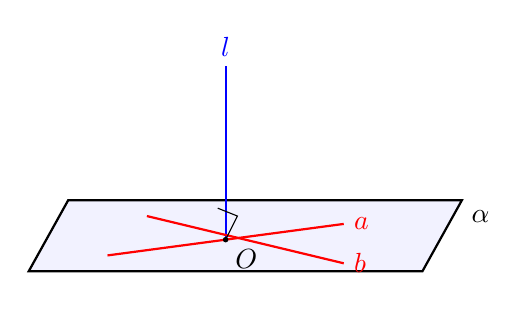
\begin{tikzpicture}[scale=1]
    \draw[thick, fill=blue!5] (-2.5, -0.4) -- (2.5, -0.4) -- (3, 0.5) -- (-2, 0.5) -- cycle;
    \coordinate (O) at (0, 0);
    \draw[thick, blue] (O) -- (0, 2.2) node[above] {$l$};
    \draw[thick, red] (-1.5, -0.2) -- (1.5, 0.2) node[right] {$a$};
    \draw[thick, red] (-1, 0.3) -- (1.5, -0.3) node[right] {$b$};
    \draw[thin] (0, 0) -- (0.15, 0.3) -- (-0.1, 0.4);
    \node at (3, 0.3) [right] {$\alpha$};
    \fill (O) circle (1pt) node[below right] {$O$};
\end{tikzpicture}
\end{center}

\section{面面垂直}

\state{面面垂直的来源}{
    \begin{enumerate}
        \item[(i)] $\blacktriangle$\ $\bc l\perp\alpha\\ l\subset\beta\ec\ \Rightarrow\ \alpha\perp\beta$（判定定理：一个面过另一个面的垂线）；
        \item[(ii)] $\bc \alpha\perp\beta\\ \alpha\parallel\gamma\ec\ \Rightarrow\ \beta\perp\gamma$。
    \end{enumerate}
}

三层之间的判定与性质，同样可以画成一张通路图：判定从上往下，性质从下往上。

\begin{center}
\begin{tikzpicture}[>=Stealth, node distance=1.5cm,
    box/.style={draw, rounded corners=1pt, minimum width=2.4cm, minimum height=0.8cm, font=\small}]
    \node[box] (ll) {线线垂直};
    \node[box, below=of ll] (lm) {线面垂直};
    \node[box, below=of lm] (mm) {面面垂直};
    \draw[->] ($(ll.south)+(-0.6,0)$) -- ($(lm.north)+(-0.6,0)$) node[midway, left] {\scriptsize 判定};
    \draw[->] ($(lm.north)+(0.6,0)$) -- ($(ll.south)+(0.6,0)$) node[midway, right] {\scriptsize 性质};
    \draw[->] ($(lm.south)+(-0.6,0)$) -- ($(mm.north)+(-0.6,0)$) node[midway, left] {\scriptsize 判定};
    \draw[->] ($(mm.north)+(0.6,0)$) -- ($(lm.south)+(0.6,0)$) node[midway, right] {\scriptsize 性质};
\end{tikzpicture}
\end{center}

\section{补充}

\subsection*{1. 三垂线定理}

\state{三垂线定理}{
    设 $P$ 为平面 $\alpha$ 外一点，$PO\perp\alpha$（$O$ 为垂足），$\ell$ 为 $\alpha$ 内一条直线。若 $OA\perp\ell$（$A$ 在 $\ell$ 上），则 $PA\perp\ell$。

    逆定理：若 $PA\perp\ell$，则 $OA\perp\ell$。
}

\begin{center}
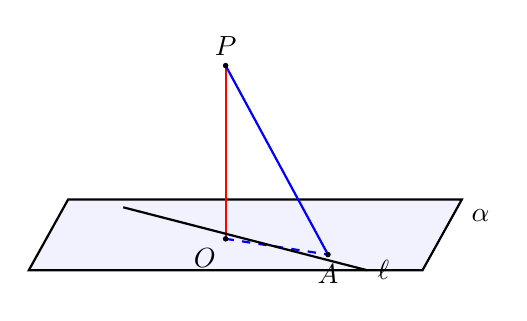
\begin{tikzpicture}[scale=1]
    \draw[thick, fill=blue!5] (-2.5, -0.4) -- (2.5, -0.4) -- (3, 0.5) -- (-2, 0.5) -- cycle;
    \coordinate (O) at (0, 0);
    \coordinate (P) at (0, 2.2);
    \coordinate (A) at (1.3, -0.2);
    \draw[thick, red] (P) -- (O);
    \draw[thick, blue] (P) -- (A);
    \draw[thick, blue, dashed] (O) -- (A);
    \draw[thick] (-1.3, 0.4) -- (1.8, -0.4) node[right] {$\ell$};
    \fill (O) circle (1pt) node[below left] {$O$};
    \fill (P) circle (1pt) node[above] {$P$};
    \fill (A) circle (1pt) node[below] {$A$};
    \node at (3, 0.3) [right] {$\alpha$};
\end{tikzpicture}
\end{center}

它把"斜线 $PA$ 与 $\ell$ 的垂直"换成平面内"射影 $OA$ 与 $\ell$ 的垂直"——平面内的垂直好判断得多。

\subsection*{2. 面面平行的简单判定}

\state{面面平行的简单判定}{
    $\bc l\perp\alpha\\ l\perp\beta\ec\ \Rightarrow\ \alpha\parallel\beta$：垂直于同一条直线的两个平面互相平行。
}

这是用垂直来证平行的一条捷径——只要找到一条直线同时垂直于两个面，两个面就平行。
